\documentclass[compress]{beamer}

\usetheme[block=fill]{metropolis}

\usepackage{graphicx} % Allows including images
\usepackage{amsmath,amsfonts,amsthm,amssymb}
\usepackage{color}
\usepackage{xcolor,cancel}
\usepackage{tcolorbox}
\setbeamercolor{colorBoxStuff}{fg=black, bg=gray!30!white}
%\setitemize{label=\usebeamerfont*{itemize item}%
%	\usebeamercolor[fg]{itemize item}
%	\usebeamertemplate{itemize item}}
\definecolor{mDarkBrown}{HTML}{604c38}
\definecolor{mDarkTeal}{HTML}{23373b}
\definecolor{mLightBrown}{HTML}{EB811B}
\definecolor{mMediumBrown}{HTML}{C87A2F}
\definecolor{mygreen}{HTML}{98C2B9}
\definecolor{myyellow}{HTML}{DFD79C}
\definecolor{myblue}{HTML}{8CA7CC}
\definecolor{kern}{HTML}{8CC2B7}


\usepackage{float}
\usepackage{framed}
\usepackage{epsfig}
\usepackage{graphicx}
\usepackage{subcaption}
\usepackage{ulem}
\usepackage{hhline}
\usepackage{multirow}
\usepackage{comment}   
\usepackage{bbm}
\usepackage{tikz}   
\def\Put(#1,#2)#3{\leavevmode\makebox(0,0){\put(#1,#2){#3}}}
\newcommand*\mystrut[1]{\vrule width0pt height0pt depth#1\relax}
\newcommand{\eqdef}{\mathbin{\stackrel{\rm def}{=}}}
\usepackage{hyperref}


\newcommand{\bs}[1]{\boldsymbol{#1}}
\newcommand{\bv}[1]{\mathbf{#1}}
\newcommand{\R}{\mathbb{R}}
\newcommand{\E}{\mathbb{E}}

\DeclareMathOperator*{\argmin}{arg\,min}
\DeclareMathOperator*{\argmax}{arg\,max}
\DeclareMathOperator{\nnz}{nnz}
\DeclareMathOperator{\vol}{vol}
\DeclareMathOperator{\diag}{diag}
\DeclareMathOperator{\Var}{Var}
\DeclareMathOperator{\sinc}{sinc}
\DeclareMathOperator{\sign}{sign}
\DeclareMathOperator{\dist}{dist}
\DeclareMathOperator{\mv}{mv}
\DeclareMathOperator{\sgn}{sgn}
\DeclareMathOperator{\step}{step}
\DeclareMathOperator{\gap}{gap}
\DeclareMathOperator{\poly}{poly}
\DeclareMathOperator{\tr}{tr}
\DeclareMathOperator{\orth}{orth}
\newcommand{\norm}[1]{\|#1\|}
\captionsetup[subfigure]{labelformat=empty}
\captionsetup[figure]{labelformat=empty}
\DeclareMathOperator*{\lmin}{\lambda_{min}}
\DeclareMathOperator*{\lmax}{\lambda_{max}}

\newcommand{\specialcell}[2][c]{%
  \begin{tabular}[#1]{@{}c@{}}#2\end{tabular}}
\newcommand{\specialcellleft}[2][c]{%
\begin{tabular}[#1]{@{}l@{}}#2\end{tabular}
}

\newtheorem{claim}[theorem]{Claim}
%\newtheorem{corollary}[theorem]{Corollary}

\usepackage{tabstackengine}
\stackMath


%----------------------------------------------------------------------------------------
%	TITLE PAGE
%----------------------------------------------------------------------------------------

\title{CS-GY 6763: Lecture 3 \\  Exponential Concentration Inequalities, Fingerprinting}
\author{NYU Tandon School of Engineering, Prof. Christopher Musco}
\date{}

\begin{document}

\begin{frame}
	\titlepage 
\end{frame}

\metroset{titleformat=smallcaps}

\begin{frame}[t]
	\frametitle{last time}
	\begin{lemma}[Chebyshev's Inequality]
		Let $X$ be a random variable with expectation $\E[X]$ and variance $\sigma^2 = \Var[X]$. Then for any $k > 0$,
		\begin{align*}
			\Pr[|X - \E[X]| \geq k\cdot\sigma] \leq \frac{1}{k^2}
		\end{align*}
	\end{lemma}
	\vspace{-.5em}
	\textbf{One application:} Proved that if you throw $n$ balls into $n$ bins, the maximum loaded bin has $O(\sqrt{n})$  balls.  We used Chebyshevs + \underline{\hspace{10em}}.
	\begin{center}
		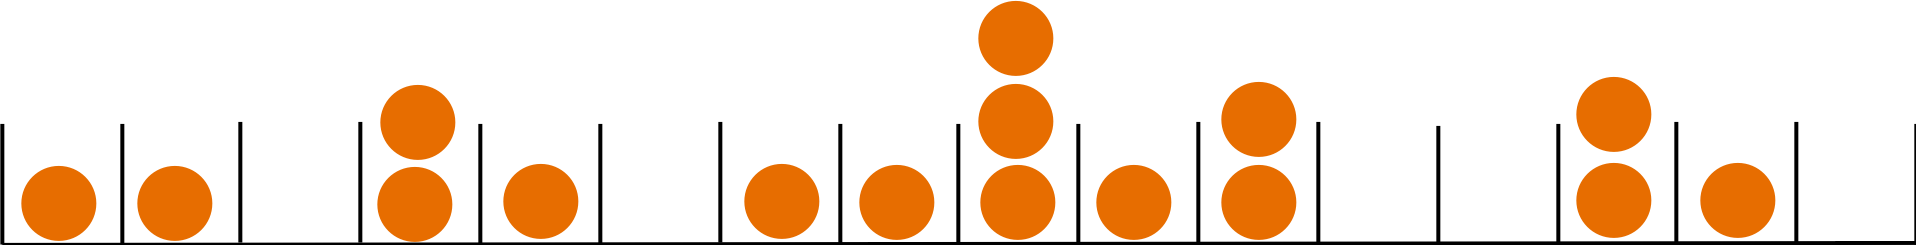
\includegraphics[width=.7\textwidth]{ballsinbins.png}
	\end{center}
This lecture, we'll prove a bound of $O(\log n)$ using stronger tools. 
\end{frame}

\begin{frame}
	\frametitle{beyond chebyshev}
	\textbf{Motivating question:} Is Chebyshev's Inequality tight?
	
	It is the worst case, but often not in reality.
	\vspace{-1em}
	\begin{figure}
		\centering
		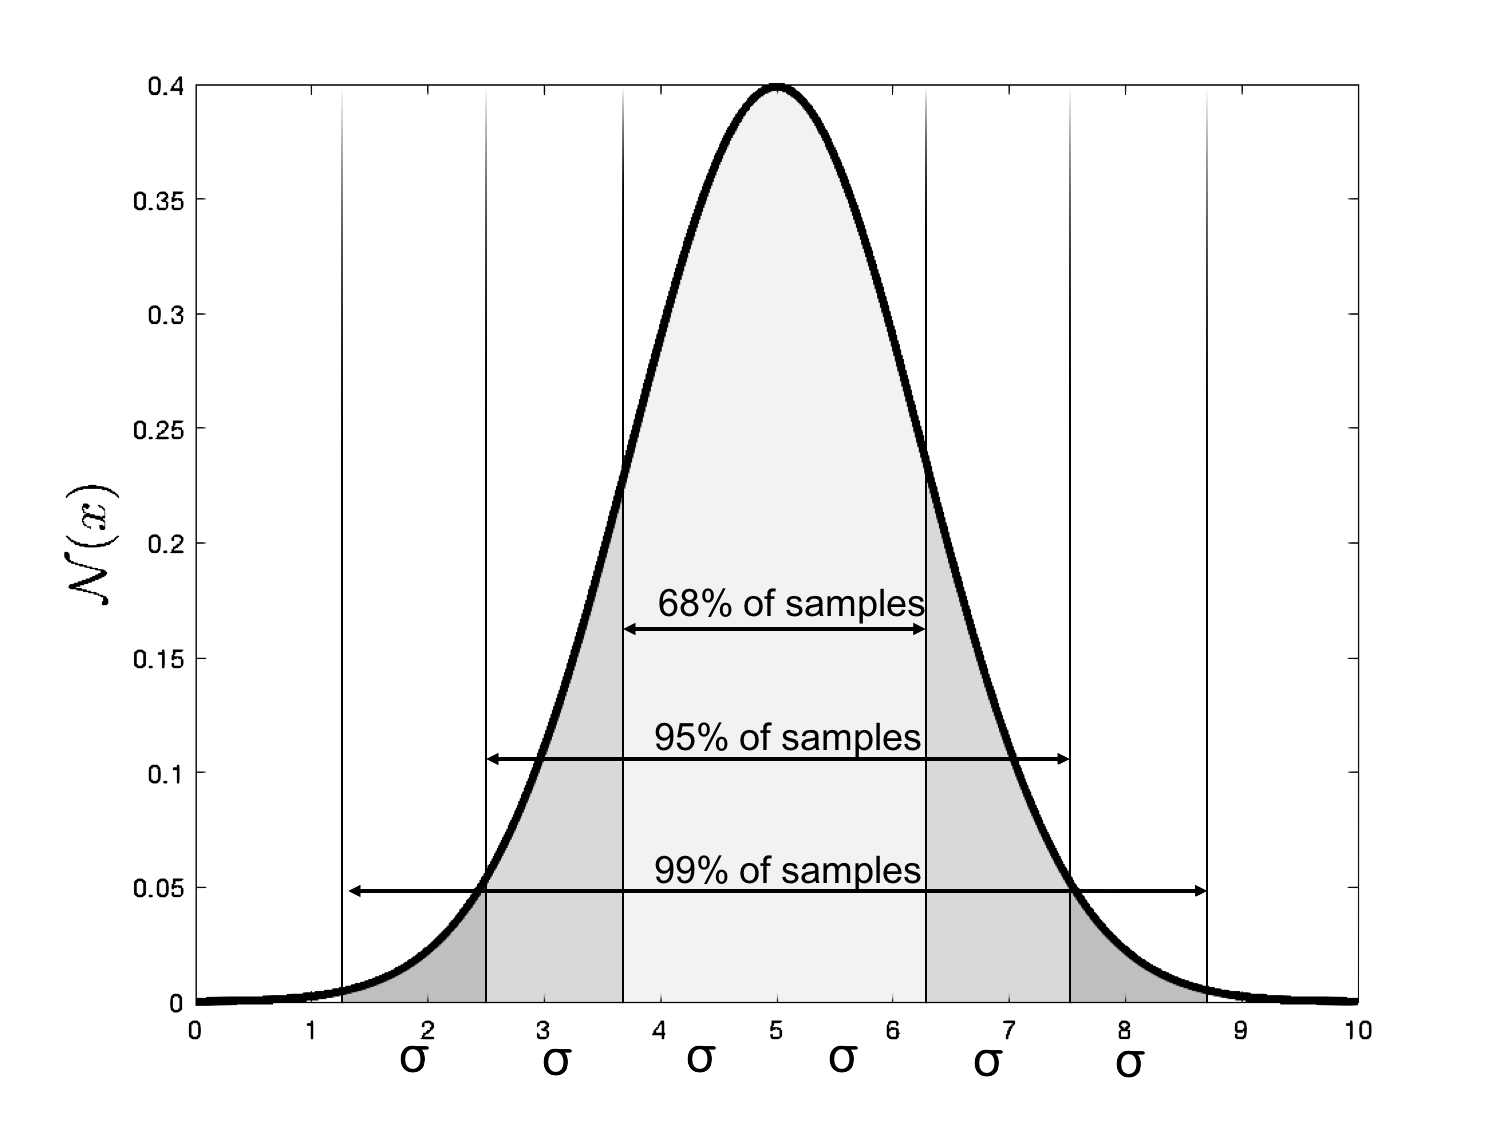
\includegraphics[width=0.4\textwidth]{689599rule.png}
		\vspace{-.5em}
		\caption{68-95-99 rule for Gaussian bell-curve. \alert{$\mathbf{X\sim N(0,\sigma^2)}$}}
	\end{figure}
	\vspace{-.5em}
	
	\begin{columns}
		\begin{column}{.5\textwidth}
			\small
			\textbf{Chebyshev's Inequality:}
			\vspace{-.5em}
			\begin{align*}
				\Pr\left(|X - \E[X]| \geq 1\sigma \right) &\leq 100\% \\
				\Pr\left(|X - \E[X]| \geq 2\sigma \right) &\leq 25\% \\
				\Pr\left(|X - \E[X]| \geq 3\sigma \right) &\leq 11\% \\
				\Pr\left(|X - \E[X]| \geq 4\sigma \right) &\leq 6\%.
			\end{align*}
		\end{column}
		\begin{column}{.5\textwidth}
			\small
			\textbf{Truth:}
			\vspace{-.5em}
			\begin{align*}
				\Pr\left(|X - \E[X]| \geq 1\sigma \right) &\approx 32\% \\
				\Pr\left(|X - \E[X]| \geq 2\sigma \right) &\approx 5\% \\
				\Pr\left(|X - \E[X]| \geq 3\sigma \right) &\approx 1\% \\
				\Pr\left(|X - \E[X]| \geq 4\sigma \right) &\approx .01\%
			\end{align*}
		\end{column}
	\end{columns}
\end{frame}

\begin{frame}
	\frametitle{gaussian concentration}
	\small
	For $X \sim \mathcal{N}(\mu,\sigma^2)$:
	\begin{align*}
		\Pr[X = \mu \pm x] \sim \frac{1}{\sigma\sqrt{2\pi}} \alert{\mathbf{e^{-x^2/2\sigma^2}}}
	\end{align*}
	\vspace{-1em}
	\begin{lemma}[Gaussian Tail Bound]
		For $X \sim \mathcal{N}(\mu,\sigma^2)$:\vspace{-.5em}
		\begin{align*}
			\Pr[|X - \E X| \geq k\cdot\sigma] \leq 2e^{-k^2/2}.
		\end{align*}
	\end{lemma}
Compare this to: 
	\begin{lemma}[Chebyshev's Inequality]
	For $X \sim \mathcal{N}(\mu,\sigma^2)$:\vspace{-.5em}
	\begin{align*}
		\Pr[|X - \E X| \geq k\cdot\sigma] \leq \frac{1}{k^2}
	\end{align*}
\end{lemma}
\end{frame}

\begin{frame}
	\frametitle{gaussian concentration}
	\begin{figure}
		\begin{subfigure}[t]{0.47\textwidth}
			\centering
			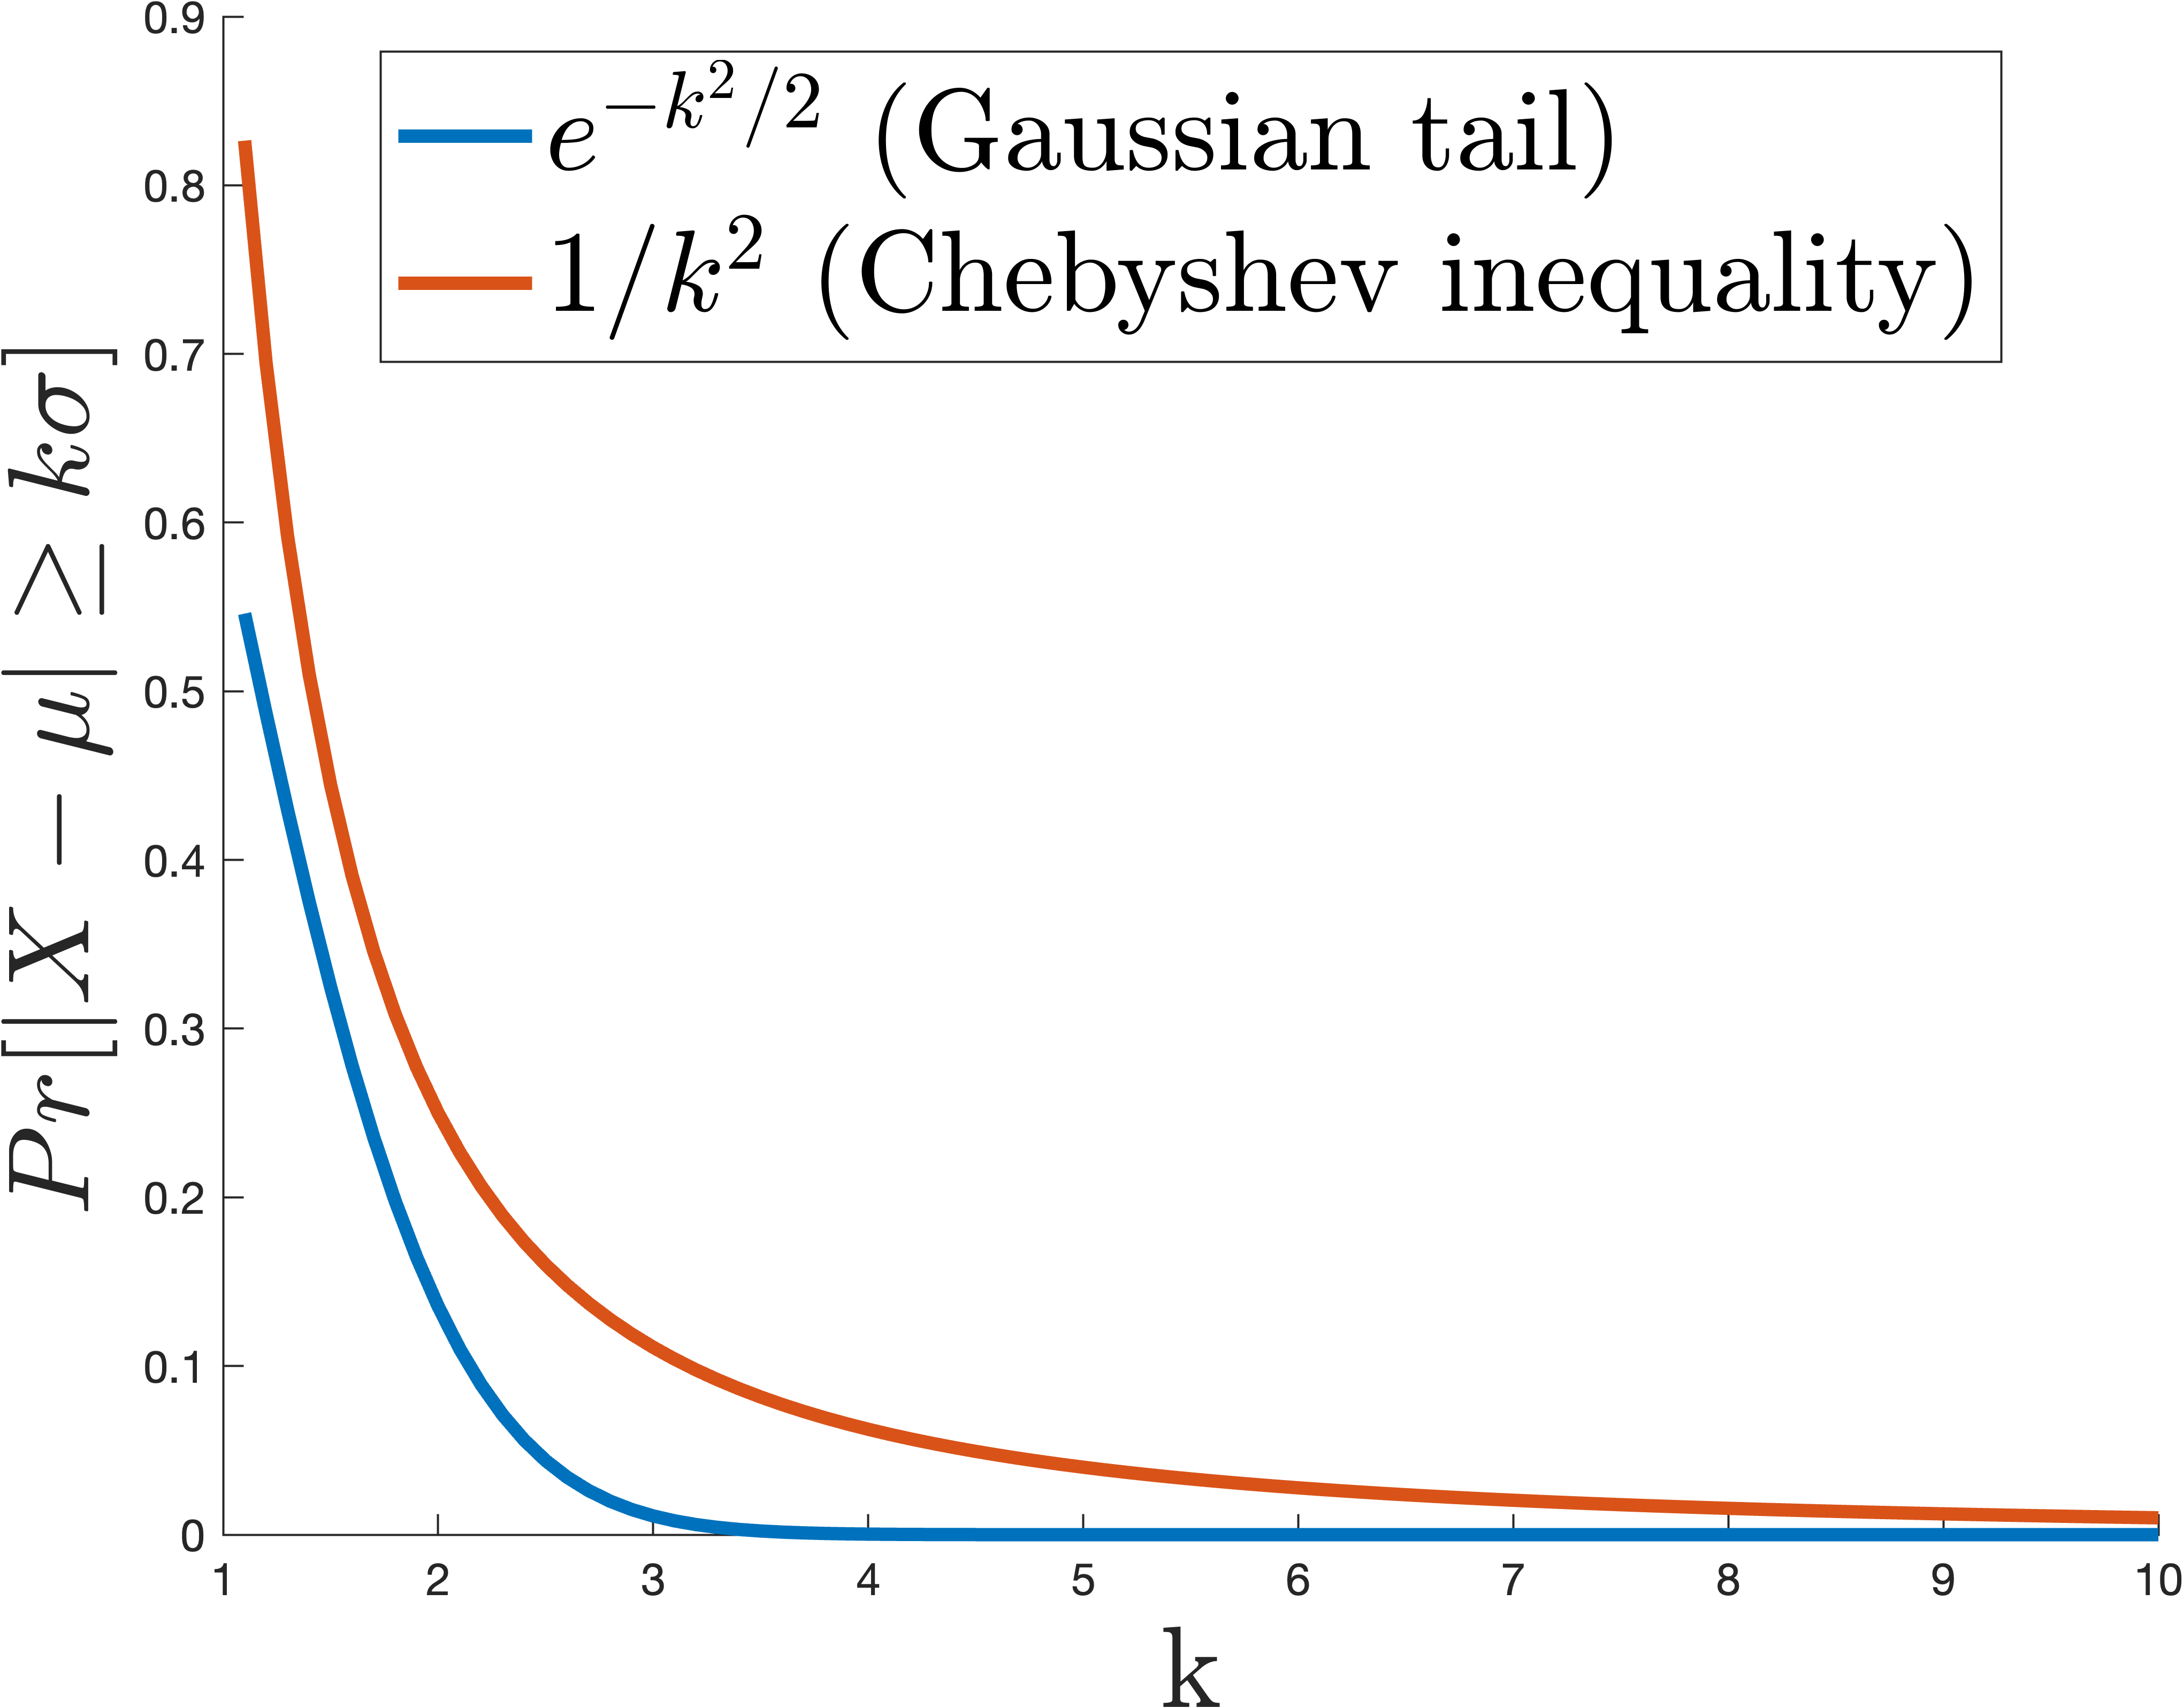
\includegraphics[width=\textwidth]{standardScale.png}
			\caption{Standard $y$-scale.}
		\end{subfigure}
		\hspace{.5em}
		\begin{subfigure}[t]{0.47\textwidth}
			\centering
			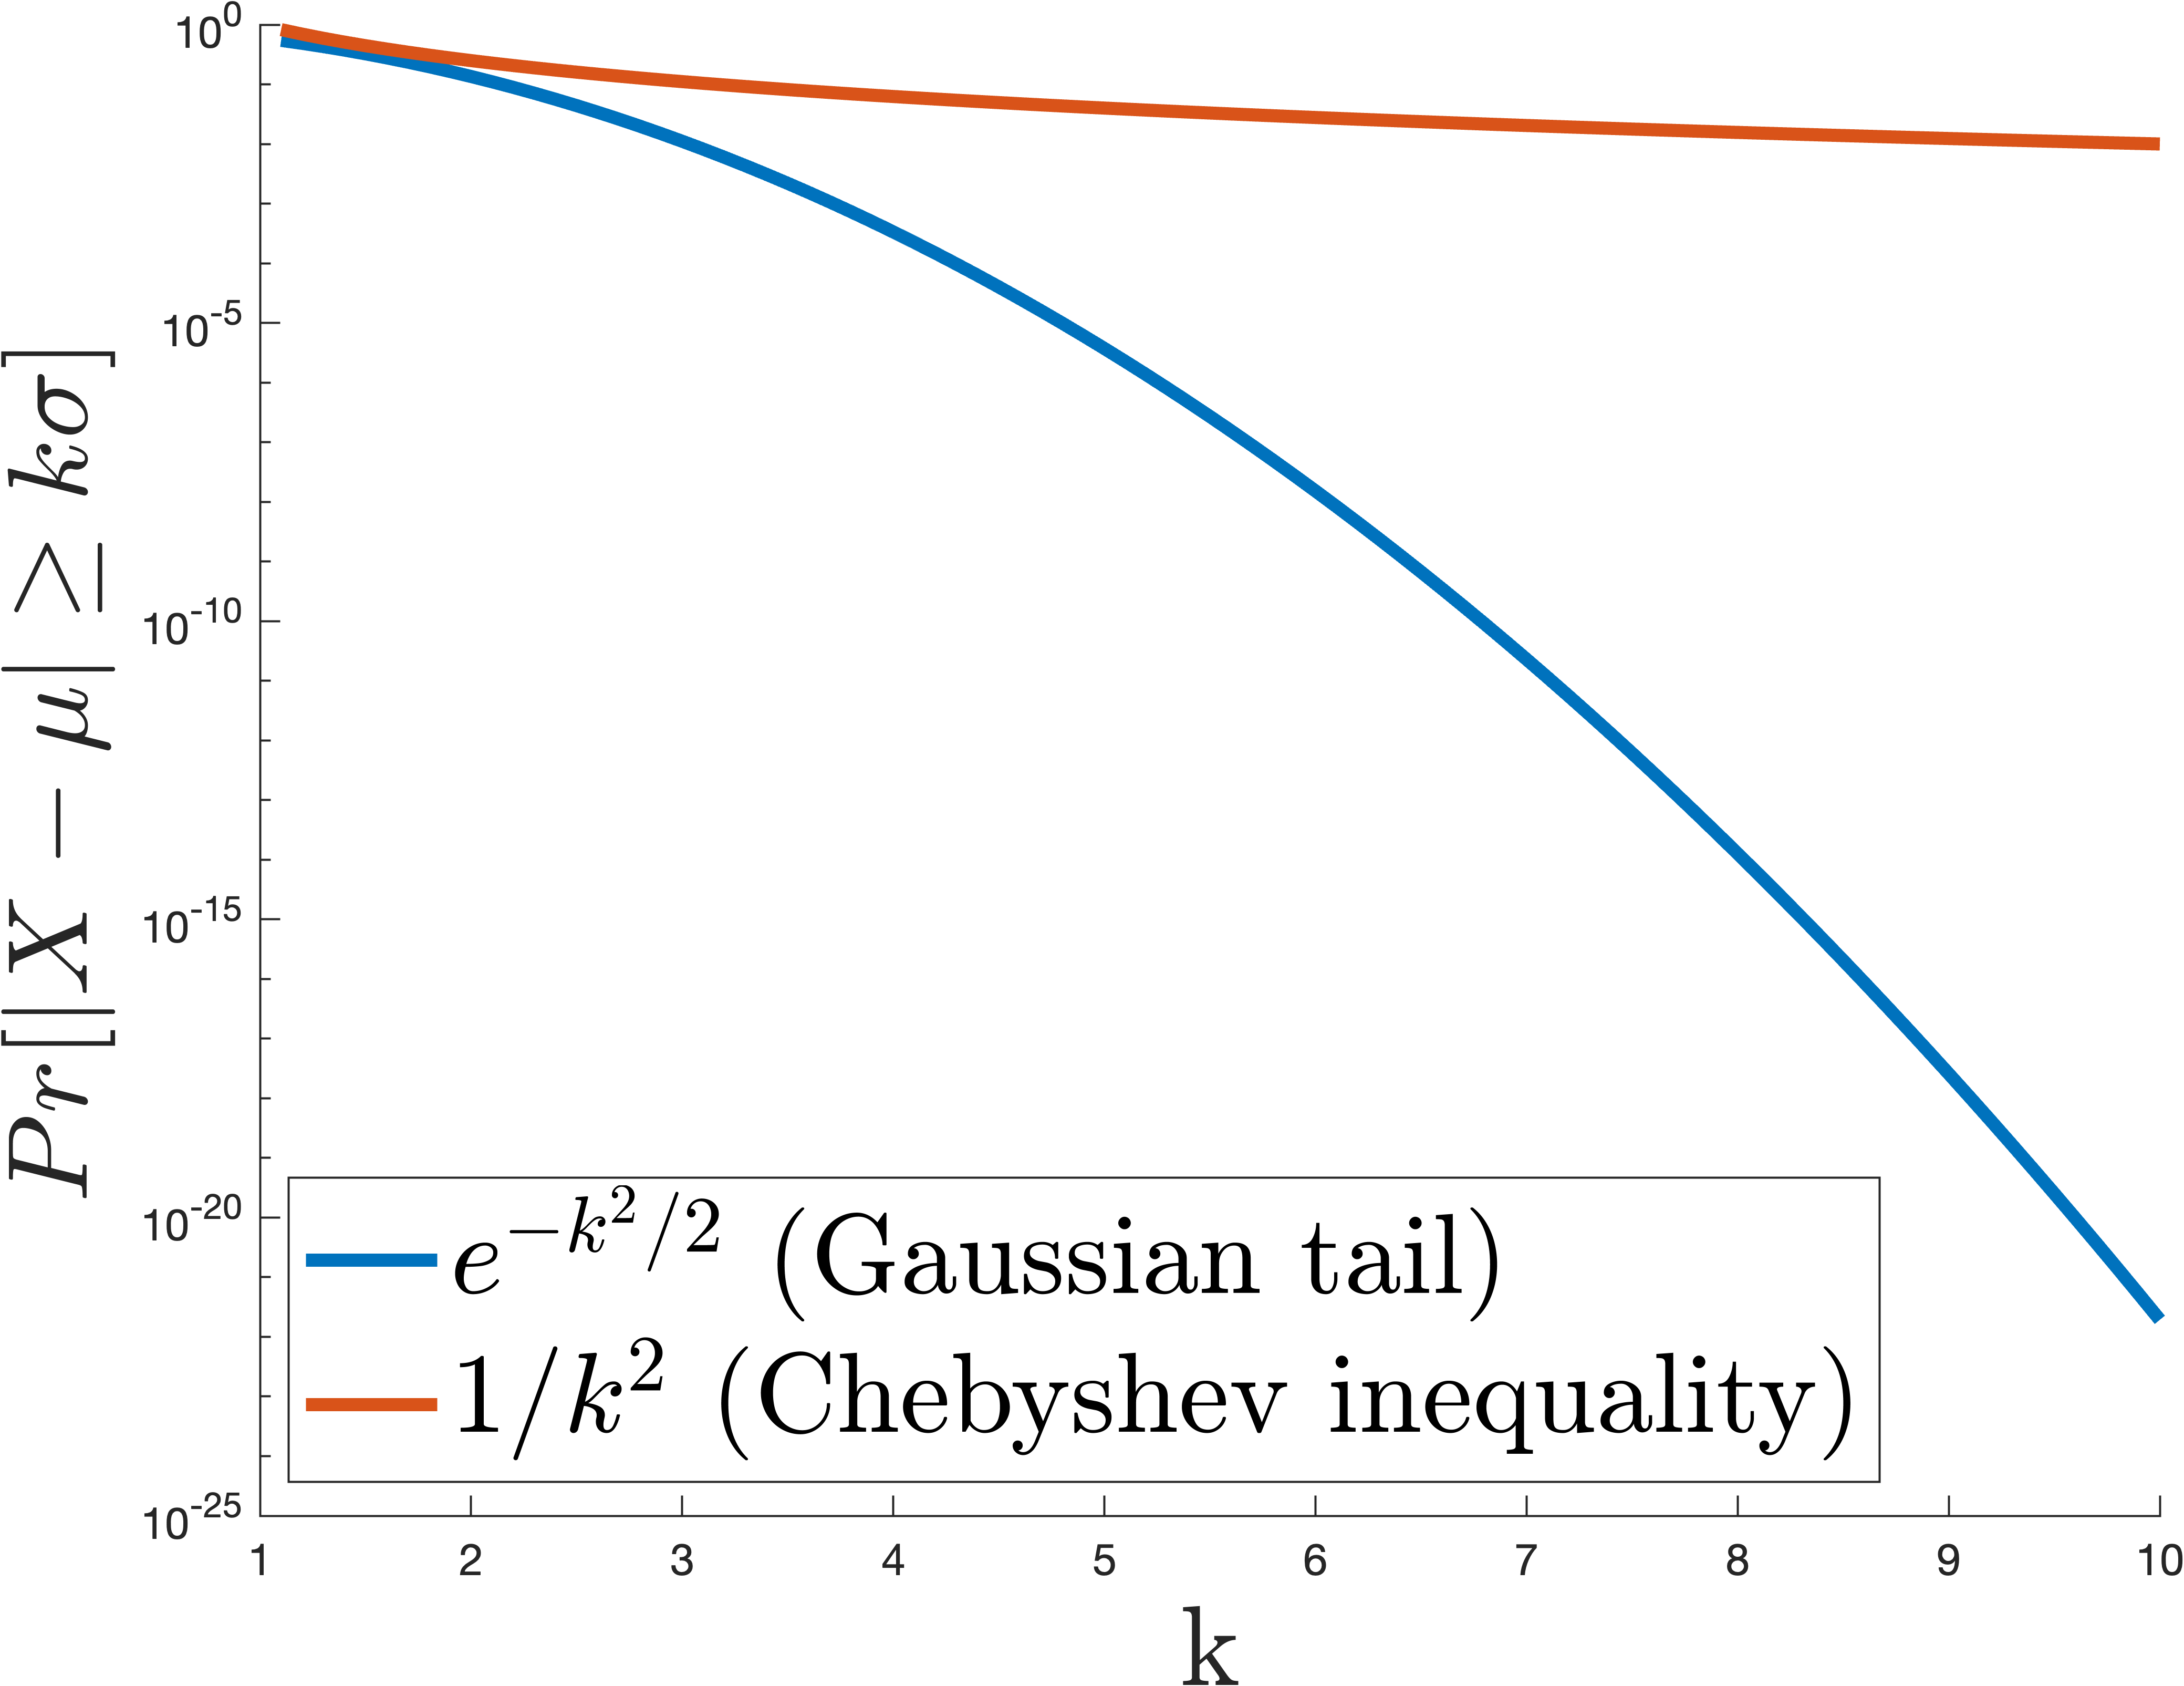
\includegraphics[width=\textwidth]{logScale.png}
			\caption{Logarithmic $y$-scale.}
		\end{subfigure}
	\end{figure}
	\textbf{Takeaway:} Gaussian random variables concentrate much tighter around their expectation than variance alone (i.e. Chebyshevs's inequality)  predicts.

\begin{center}
	\alert{\textbf{Why does this matter for algorithm design?}}
\end{center}
\end{frame}

\begin{frame}
	\frametitle{central limit theorem}
	\begin{theorem}[CLT -- Informal]
		Any sum of \alert{mutually independent}, \alert{(identically distributed)}  r.v.'s $X_1,  \ldots, X_k$ with mean $\mu$ and finite variance $\sigma^2$ converges to a Gaussian r.v. with mean $k\cdot\mu$ and variance $k\cdot\sigma^2$, as $k\rightarrow \infty$.
		\vspace{-.5em}
		\begin{align*}
			S = \sum_{i=1}^n X_i \Longrightarrow \mathcal{N}(k\cdot\mu, k\cdot\sigma^2).
		\end{align*}	
		\vspace{-.5em}	
	\end{theorem}
	\vspace{-.5em}	
	\begin{figure}
		\begin{subfigure}[t]{0.4\textwidth}
			\centering
			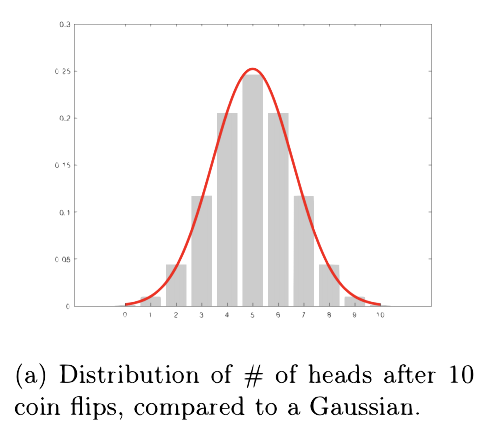
\includegraphics[width=\textwidth]{cltWide.png}
		\end{subfigure}
		\hspace{4em}
		\begin{subfigure}[t]{0.4\textwidth}
			\centering
			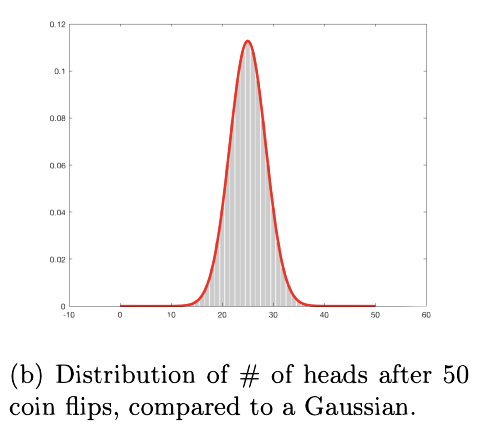
\includegraphics[width=\textwidth]{cltSkinny.png}
		\end{subfigure}
	\end{figure}
\end{frame}

\begin{frame}
	\frametitle{independence}
	Recall:
	\vspace{1em}
	\begin{definition}[Mutual Independence]
		Random variables $X_1, \ldots, X_k$ are \emph{mutually independent} if, for all possible values $v_1, \ldots, v_k$,
		\begin{align*}
			\Pr[X_1 = v_1, \ldots, X_k = v_k] = 	\Pr[X_1 = v_1]\cdot\ldots \cdot\Pr[X_k = v_k]
		\end{align*}
	\end{definition}
	\begin{center}
		\textbf{Strictly stronger than pairwise independence.}
	\end{center}
\end{frame}

\begin{frame}
	\frametitle{exercise}
	\small 
	\begin{center}
		\textbf{If I flip a fair coin $100$ times, lower bound the chance I get between $30$ and $70$ heads?}
	\end{center}
	%	As in the previous lecture, we we would like to use concentration bounds to study the randomized load balancing problem. $n$ jobs are distributed randomly to $n$ servers using a hash function. Let $S_i$ be the number of jobs sent to server $i$. 
	%	\begin{enumerate}[label=(\alph*)]
		%		\item Using the CLT and our lemma for Gaussian concentration, estimate a bound for $\max_i[S_i]$. For example, your bound should take the form: $\Pr[max_i S_i \geq \alert{\textbf{B}}] \leq 1/10$. What's the smallest value of $\textbf{\alert{B}}$ you should hope to achieve? 
		%		\item Last class we proved the above bound with $\textbf{B} = O(\sqrt{n})$ using Chebyshev inequality. How does your bound compare?
		%	\end{enumerate}
	
	For this problem, we will assume the limit of the CLT holds \emph{exactly} -- i.e., that this sum looks exactly like a Gaussian random variable.
	\begin{lemma}[Gaussian Tail Bound]
		For $X \sim \mathcal{N}(\mu,\sigma^2)$:\vspace{-.5em}
		\begin{align*}
			\Pr[|X - \E X| \geq k\cdot\sigma] \leq 2e^{-k^2/2}.
		\end{align*}
	\end{lemma}
	\vspace{3em}
	$2e^{-8} = .06\%$. Chebyshev's inequality gave a bound of $6.25\%$. 
\end{frame}

%\begin{frame}
%	\frametitle{back-of-the-envelop calculation}
%	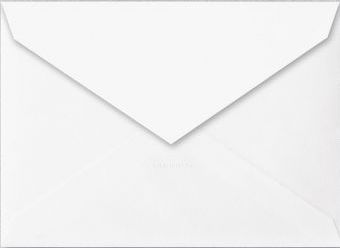
\includegraphics[width=.9\textwidth]{envelope.jpg}
%\end{frame}


\begin{frame}
	\frametitle{quantitative versions of the clt}
	\textbf{These back-of-the-envelop calculations can be made rigorous!}
	\textbf{\alert{Lots of different ``versions'' of bound which do so.}}
		\begin{center}
			\begin{itemize}
				\item Chernoff bound
				\item Bernstein bound
				\item Hoeffding bound
				\item $\ldots$
			\end{itemize}
			Different assumptions on random varibles (e.g. binary vs. bounded), different forms (additive vs. multiplicative error), etc. \textbf{Wikipedia is your friend.}
		\end{center}
\end{frame}

\begin{frame}
	\frametitle{quantitative versions of the clt}
	\begin{theorem}[Chernoff Bound]
		Let $X_1,X_2,\ldots,X_k$ be independent $\{0,1\}$-valued random variables and let
		$p_i = \E[X_i]$, where $0<p_i<1$.
		Then the sum $S = \sum_{i=1}^{k} X_i$, which has mean
		$\mu = \sum_{i=1}^{k} p_i$, satisfies
		\begin{align*}
			\Pr[S \geq (1+\epsilon)\mu] \leq e^{\frac{-\epsilon^2\mu}{2+ \epsilon}}.
		\end{align*}
		and for $0<\epsilon <1$
		\begin{align*}
			\Pr[S \leq (1-\epsilon)\mu] \leq e^{\frac{-\epsilon^2\mu}{2}}.
		\end{align*}
	\end{theorem} 
\end{frame}

\begin{frame}[t]
	\frametitle{chernoff bound}
	\begin{theorem}[Chernoff Bound Corollary]
		Let $X_1,X_2,\ldots,X_k$ be independent $\{0,1\}$-valued random variables and let
		$p_i = \E[X_i]$, where $0<p_i<1$.
		Let $S = \sum_{i=1}^{k} X_i$ and $\E[S] = \mu$. For $\epsilon \in (0,1)$,
		\begin{align*}
				\Pr[|S - \mu| \geq \epsilon \mu] \leq 2e^{-\epsilon^2 \mu/3}
		\end{align*}
	\end{theorem} 
Why does this look like the Gaussian tail bound of 	$\Pr[|S - \mu| \geq k\cdot\sigma] \lesssim 2e^{-k^2/2}$? What is $\sigma(S)$?
\end{frame}



\begin{frame}[t]
	\frametitle{quantitative versions of the clt}
	\begin{theorem}[Bernstein Inequality]
		Let $X_1, X_2, \ldots, X_k$ be independent random variables with each $X_i \in [-1,1]$.
		Let $\mu_i =\E[X_i]$ and $\sigma_i^2 = \Var[X_i]$. Let  $\mu =\sum_i \mu_i$ and $\sigma^2 =\sum_i \sigma_i^2$. Then, for $k \leq \frac{1}{2}\sigma$, $S =\sum_i X_i$ satisfies
		$$\Pr[|S - \mu| > k\cdot \sigma] \leq  2 e^{-{k^2}/{4}}.$$
	\end{theorem}
\end{frame}

\begin{frame}[t]
	\frametitle{quantitative versions of the clt}
	\begin{theorem}[Hoeffding Inequality]
		Let $X_1, X_2, \ldots, X_k$ be independent random variables with each $X_i \in [a_i,b_i]$.
		Let $\mu_i =\E[X_i]$ and $\mu =\sum_i \mu_i$. Then, for any $k > 0$, $S =\sum_i X_i$ satisfies:
		$$\Pr[|S - \mu| > k] \leq  2 e^{-\frac{k^2}{\sum_{i=1}^k (b_i-a_i)^2}}.$$
	\end{theorem}
\end{frame}

\begin{frame}
	\frametitle{how are these bounds proven?}
	Variance is a natural \emph{measure of central tendency}, but there are others. 
	\begin{align*}
		q^\text{th} \text{ central moment: } \E[(X-\E X)^q]
	\end{align*}
	$q = 2$ gives the variance. Proof of Chebyshev's applies Markov's inequality to the random variable $(X - \E X)^2)$.
	
	\textbf{Idea in brief:} Apply Markov's inequality to $\E[(X-\E X)^q]$ for larger $q$, or more generally to $f(X-\E X)$ for some other non-negative function $f$. E.g., to $\exp(X-\E X)$. 
\end{frame}

\begin{frame}[t]
	\frametitle{exercise}
	\small 
	\begin{center}
		\textbf{If I flip a fair coin $100$ times, lower bound the chance I get between $30$ and $70$ heads?}
	\end{center}
	
		\textbf{Corollary of Chernoff bound}: Let $S = \sum_{i=1}^k X_i$ and $\mu = \E[S]$. For $0< \epsilon < 1$, 
	\vspace{-.75em}
	\begin{align*}
		\Pr[|S - \mu| \geq \epsilon \mu] \leq 2e^{-\epsilon^2 \mu/3}
	\end{align*} 
	Here $X_i = \mathbbm{1}[i^\text{th} \text{ flip is heads}]$. 
	\vspace{3em}
	
	$1.4\%$.
\end{frame}

\begin{frame}[t]
	\frametitle{chernoff bound application}
	\textbf{General Statement:} Flip biased coin $k$ times: i.e. the coin is heads with probability $b$. As long as $k \geq O\left(\frac{\log(1/\delta)}{\epsilon^2}\right)$,
	\vspace{-.5em}
	\begin{align*}
		\Pr[|\text{\# heads} - b\cdot k| \geq \epsilon k] \leq \delta 
	\end{align*}

	

	\vspace{10em}
		Pay very little for higher probability -- if you increase the number of coin flips by 4x, $\delta$ goes from $1/10 \rightarrow 1/100 \rightarrow 1/10000$
\end{frame}


%\begin{frame}
%	\frametitle{application to minhash}
%	Let $J = J(\bv{q},\bv{y})$ denote the true Jaccard similarity.
%	
%	\textbf{Estimator:} $\tilde{J} = \frac{1}{k} \sum_{i=1}^k \mathbbm{1}[c_i(\bv{q}) = c_i(\bv{y})]$. 
%	
%	By the analysis above,
%	\begin{align*}
	%		\Pr[|\tilde{J} - J| \geq \epsilon] = \Pr[|\tilde{J} \cdot k - J\cdot k| \geq \epsilon k] \leq \delta 
	%	\end{align*} 
%	as long as $k = O\left(\frac{\log(1/\delta)}{\epsilon^2}\right)$. 
%	
%	Much better than the $k = O\left(\frac{1}{\delta\epsilon^2}\right)$.
%	
%	For example, if we had a data base of $n=1,000,000$ songs, setting $\delta = \frac{1}{n}$ would only require space depending on $\log(n) \approx 14$, instead of on $n=1,000,000$.  
%	
%\end{frame}


\begin{frame}
	\frametitle{load balancing}
	\small
	\textbf{Recall:} $n$ jobs are distributed randomly to $n$ servers using a hash function. Let $S_i$ be the number of jobs sent to server $i$.  What's the smallest $\alert{\mathbf{B}}$ for which we can prove:
	\begin{align*}
		\Pr[\max_i S_i \geq \alert{\mathbf{B}}] \leq 1/10
	\end{align*}
	\vspace{-1em}
	\begin{center}
		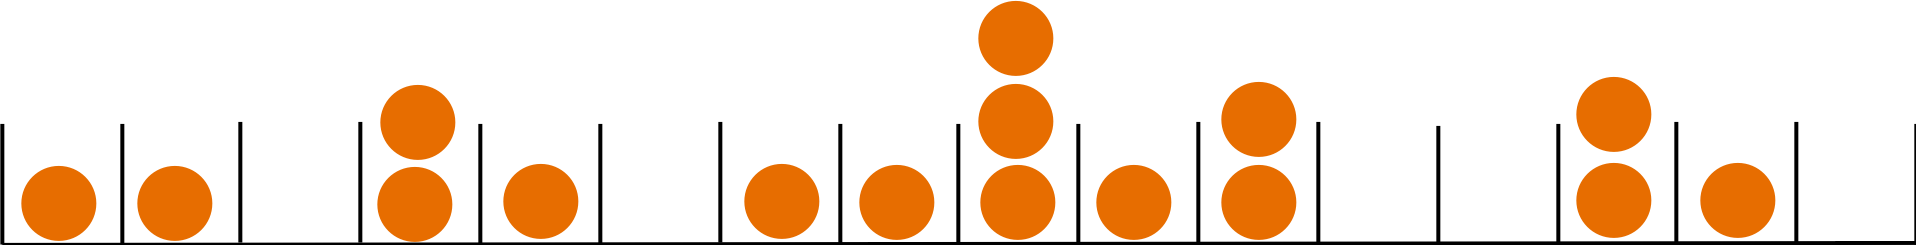
\includegraphics[width=.6\textwidth]{ballsinbins.png}
	\end{center}
	
	\textbf{Recall:} Suffices to prove that, for any $i$, $\Pr[ S_i \geq {\mathbf{B}}] \leq 1/10n$:
	\begin{align*}
		\Pr[\max_i S_i \geq {\mathbf{B}}] &= \Pr[S_1 \geq {\mathbf{B}} \text{ or } \ldots \text{ or } S_1 \geq {\mathbf{B}}] \\
		&\leq \Pr[S_1 \geq {\mathbf{B}}] + \ldots + \Pr[S_n \geq {\mathbf{B}}] \text{\hspace{1em} (union bound)}.
	\end{align*}
\end{frame}

\begin{frame}[t]
	\frametitle{load balancing}
	\begin{theorem}[Chernoff Bound]
		Let $X_1,X_2,\ldots,X_n$ be independent $\{0,1\}$-valued random variables and let
		$p_i = \E[X_i]$, where $0<p_i<1$.
		Then the sum $S = \sum_{j=1}^{n} X_i$, which has mean
		$\mu = \sum_{j=1}^{n} p_i$, satisfies
		\begin{align*}
			\Pr[X \geq (1+\epsilon)\mu] \leq e^{\frac{-\epsilon^2\mu}{2+ \epsilon}}.
		\end{align*}
	\end{theorem} 
	Consider a single bin. Let $X_j = \mathbbm{1}[\text{ball $j$ lands in that bin}]$. \vspace{2em}
	\begin{align*}
		\Pr[S \geq (1+c\log n)\mu] \leq e^{\frac{-c^2\log^2 n}{2 + c\log n}} \leq e^{\frac{-c\log^2 n}{2\log n}} \leq e^{-.5c\log n} \leq \frac{1}{10n},
	\end{align*}
	for sufficiently large $c$
	
\end{frame}

\begin{frame}
	\frametitle{load balancing}
	\begin{center}\alert{\textbf{So max load for randomized load balancing is $O(\log n)$!}} Best we could prove with Chebyshev's was $O(\sqrt{n})$. \end{center}
\end{frame}

\begin{frame}
	\frametitle{power of two choices}
	\textbf{Power of 2 Choices:} Instead of assigning job to random server, choose 2 random servers and assign to the least loaded. With probability $1/10$ the maximum load is bounded by:
	
	(a) $O(\log n)$ \hspace{1em} (b) $O(\sqrt{\log n})$  \hspace{1em}  (c) $O(\log \log n)$  \hspace{1em} (d) $O(1)$
	\begin{center}
		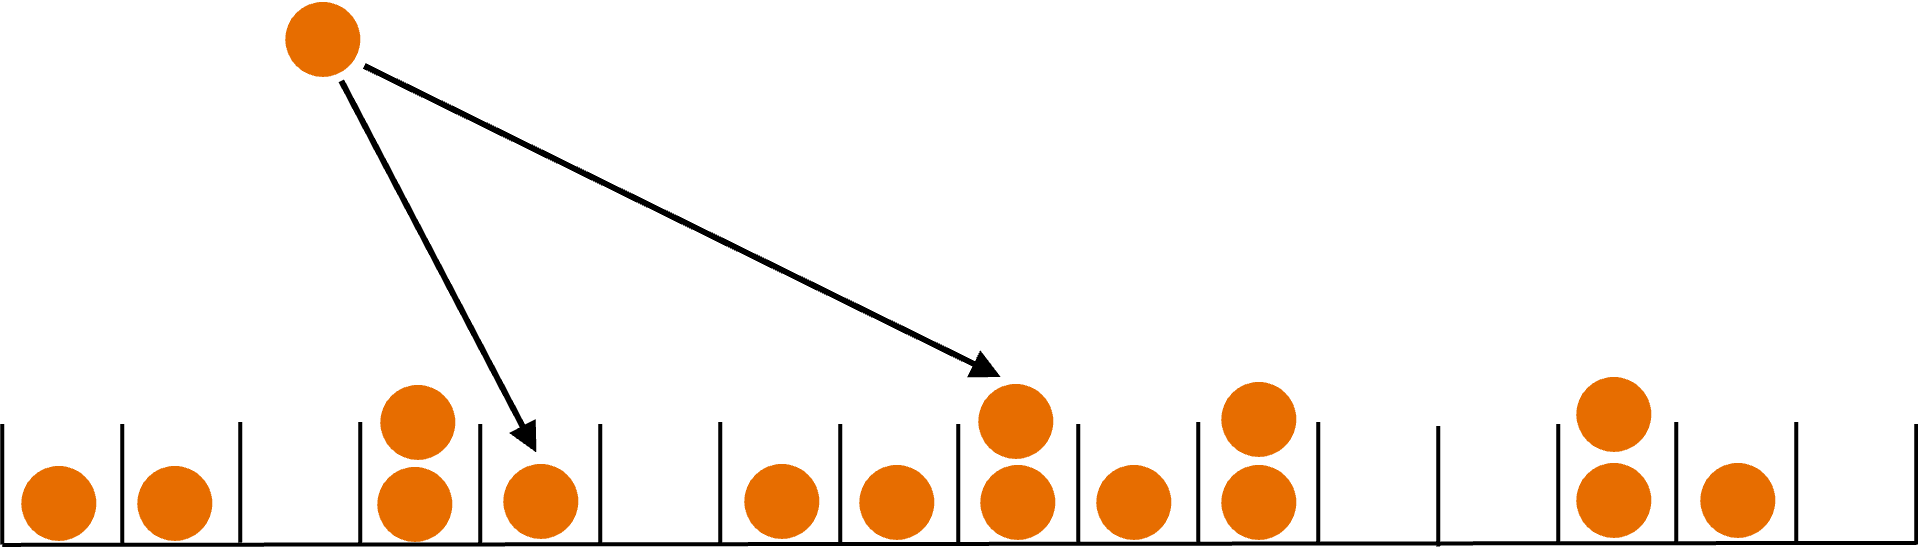
\includegraphics[width=.9\textwidth]{power_of_two.png}
	\end{center}
\end{frame}

\begin{frame}[standout]
	\begin{center}
		break
	\end{center}
\end{frame}

	\begin{frame}
	\frametitle{pseudorandom hash functions}
	\textbf{Recall from last class:}
	\begin{definition}[Universal hash function]
		 A random hash function $h: \mathcal{U} \rightarrow \{1, \ldots, m\}$ is \emph{universal} if, for any fixed $x,y\in \mathcal{U}$,\vspace{-1.5em}
		\begin{align*}
			\Pr[h(x) = h(y)] \leq \frac{1}{m}.
		\end{align*}
	\end{definition}
	\textbf{Efficient construction:} Let $p$ be a prime number between $|\mathcal{U}|$ and $2|\mathcal{U}|$. Let $a,b$ be random numbers in $0,\ldots, p$, $a\neq 0$.
	\begin{align*}
		h(x) = \left[a\cdot x + b \pmod{p}\right] \pmod{m}
	\end{align*} 
	is universal. 
	
	\begin{center}
\textbf{We're not going to prove this, but this year I want to give a flavor for what tools are used.}
	\end{center}
\end{frame}


\begin{frame}
	\frametitle{prime number checking}
	\begin{center}
		\textbf{\alert{One of the most famous applications of randomness in algorithm design.}}
	\end{center}
	\textbf{Computational Problem:} Given a number $x$, is $x$ prime? 
	
	\textbf{Recall:} 
	\begin{itemize}
		\item A number is prime if it can only be divided evenly by $1$ and itself. 
		\item The first few primes are $2,3,5,7,11,13, 17, 19,\ldots$.
		\item Is 2023 prime?
		\item What about 49301977064557719291?
	\end{itemize}
	\textbf{How would you design a generic algorithm to check?}
\end{frame}

\begin{frame}
	\frametitle{prime number checking}
	Suppose we have an integer represented as a length $n$ binary string. 
	\begin{align*}
		x = 0110100010110101\ldots1010001110
	\end{align*}
The naive prime checking algorithm runs in $O(2^n)$ time. 

NYU Greene Super Computer has $~ 2$ petaFLOPS of throughput. When $n = 128$, would need 1 million Greene Super computers running for 1 million years to check is $x$ is prime. 
\end{frame}

\begin{frame}
	\frametitle{randomized primality test}
	\textbf{Miller-Rabin 1976, 1980:} There is a \emph{randomized} algorithm running in $O(n^3 \log_2(1/\delta))$ time that, with probability $1-\delta$ determines if an $n$-bit integer $x$ is prime.  
	\begin{itemize}
		\item $n = 128$
		\item $\delta = 10^{-9}$ (chance of winning the Powerball Jackpot)
		\item $n^3\log_2(1/\delta) \approx 60$ million operations.
	\end{itemize}
	Could check in $< .1$ second on my laptop.
	\begin{center}
		\large \alert{\textbf{This was a really big break through!}}
	\end{center}
\end{frame}

\begin{frame}
	\frametitle{randomized primality test}
	Took over 20 more years to find a \emph{deterministic} polynomial time primality test.
	\begin{center}
		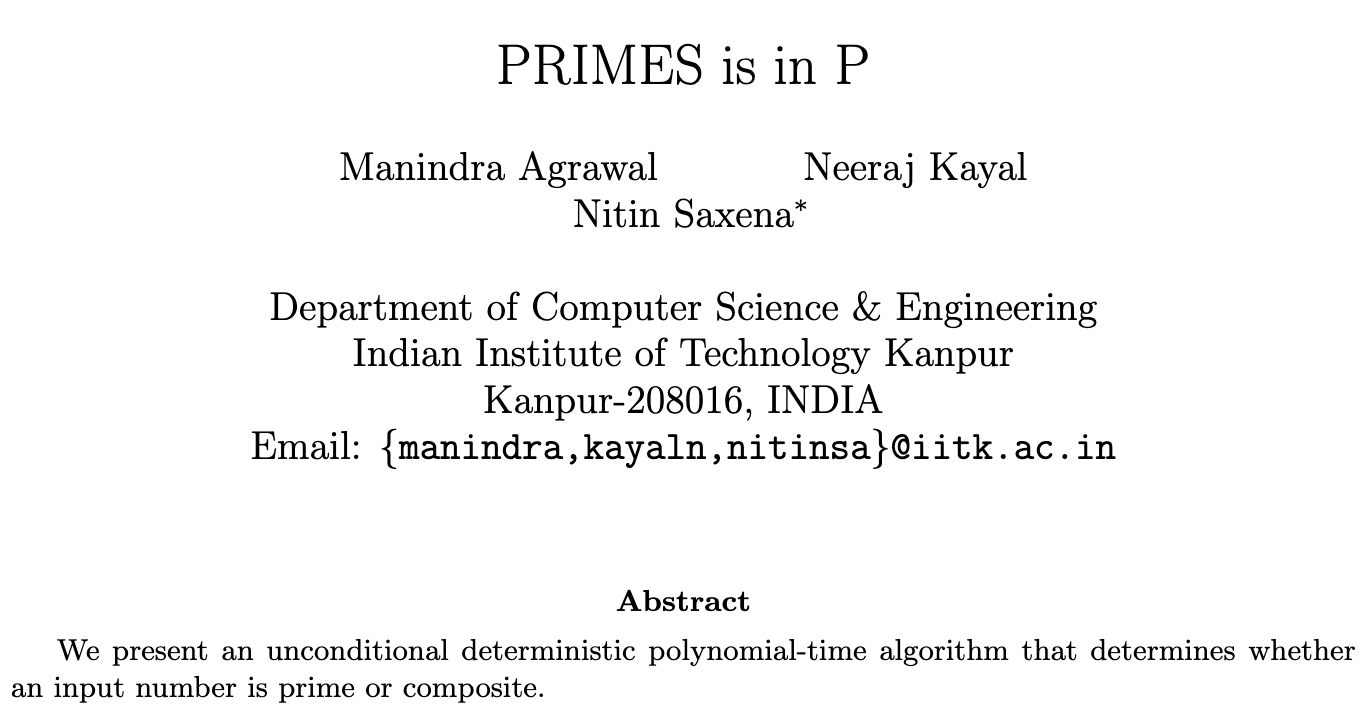
\includegraphics[width=\textwidth]{primes_in_p.png}
	\end{center}
\end{frame}

\begin{frame}
	\frametitle{why do primes matter?}
	Basis for modern public-key cryptography.
	
	\textbf{Goal:} Bob wants to send Alice an email. Wants to \textbf{\alert{encrypt}} it in some way so that even if it is intercepted, no one can read it besides Alice.
	
	\begin{center}
		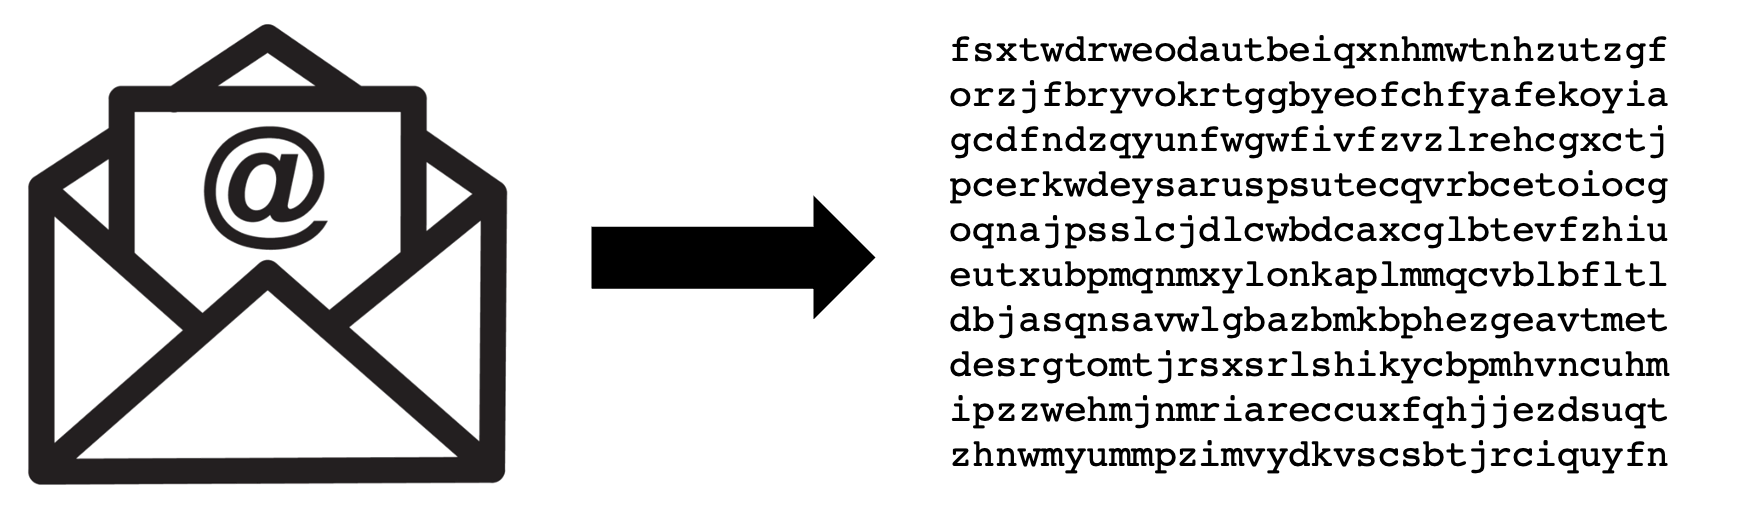
\includegraphics[width=.9\textwidth]{encrypted_message.png}
	\end{center}
\end{frame}

\begin{frame}
	\frametitle{why do primes matter?}
	Basis for modern public-key cryptography.
	
	\textbf{Goal:} Bob wants to send Alice an email. Wants to \textbf{\alert{encrypt}} it in some way so that even if it is intercepted, no one can read it besides Alice.
	
	\textbf{Option 1:} Share some sort of secret key/codebook in advance.
	\begin{center}
		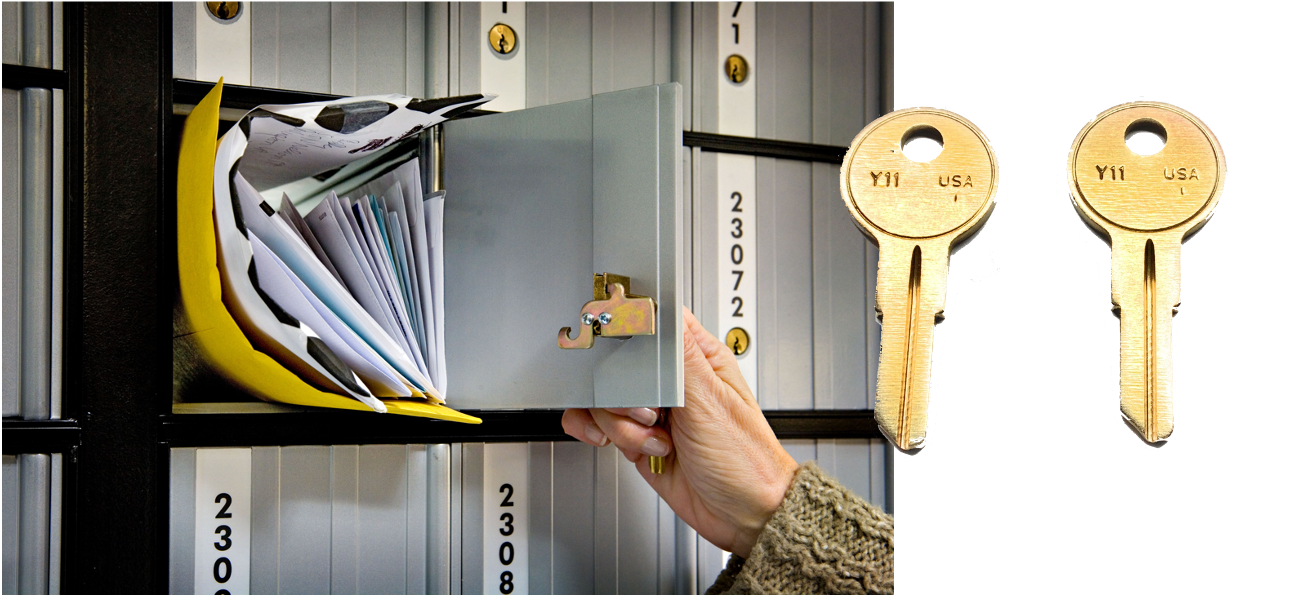
\includegraphics[width=.6\textwidth]{share_key.png}
	\end{center}
	Impractical if you have a large number of uncoordinated senders and receivers. 
\end{frame}

\begin{frame}
	\frametitle{ public-key cryptography}
	\textbf{Option 2:} Create a 1-way lock box.
	\begin{center}
		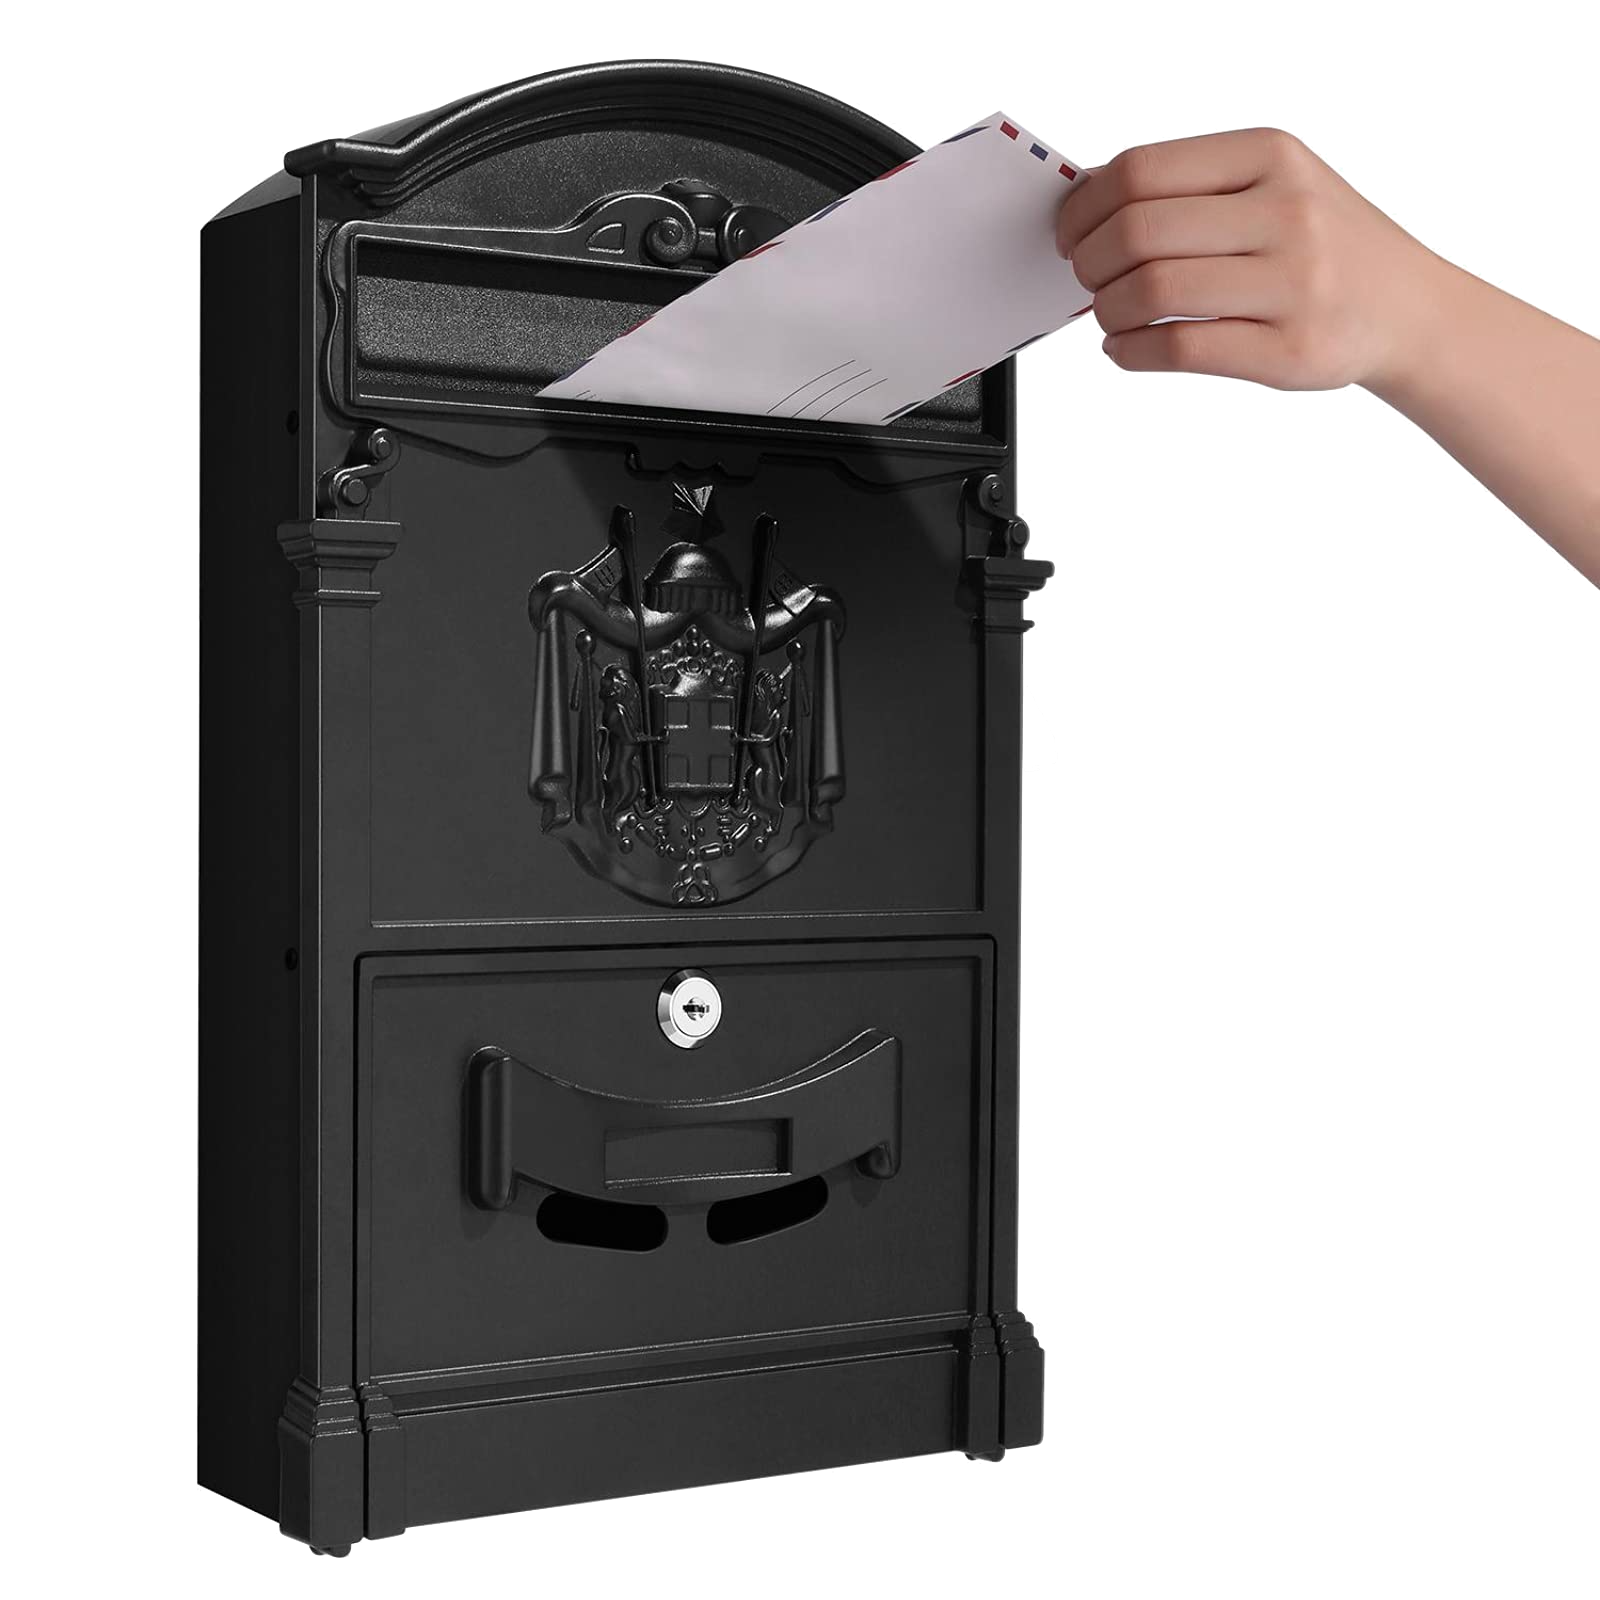
\includegraphics[width=.4\textwidth]{locking_mailbox.png}
	\end{center}
	Anyone can deliver, only Alice can open/read the messages.
\end{frame}

\begin{frame}
	\frametitle{why do primes matter?}	
	RSA crytosystem (Rivest, Shamir, Adleman 1977): 
	\begin{itemize}
		\item \textbf{Private key:} Two large (e.g. 128 bit) prime numbers $p,q$.
		\item \textbf{Public key:} Based on $z = p\times q$.  
	\end{itemize} 
	
	Even though checking if a number of prime can be done quickly, we do not have efficient algorithms for factoring numbers. E.g. for finding $p,q$ based on $z$.\footnote{At least on classical computers we don't... different story on quantum computers.}
\end{frame}


\begin{frame}
	\frametitle{from prime testing to prime generation}
	\textbf{How to find a 128 bit prime number $p$?} \alert{\textbf{Use randomness, twice.}}
	\begin{itemize}
		\item Pick a random 128 bit number. 
		\item Check if it's prime (using randomized primality test).
		\item If not, repeat.
	\end{itemize}
	\begin{center}
		\emph{Roughly how many tries do you expect this to take?}
	\end{center}
\end{frame}

\begin{frame}
	\frametitle{prime number theorem}
 Let $\pi(x)$ denote the number of primes less than some integer $x$. 	\textbf{Informally:}
	\vspace{-.5em}
	\begin{align*}
		\pi(x) \sim \frac{x}{\log(x)}
	\end{align*}
	\vspace{-1em}
	
	\begin{center}
		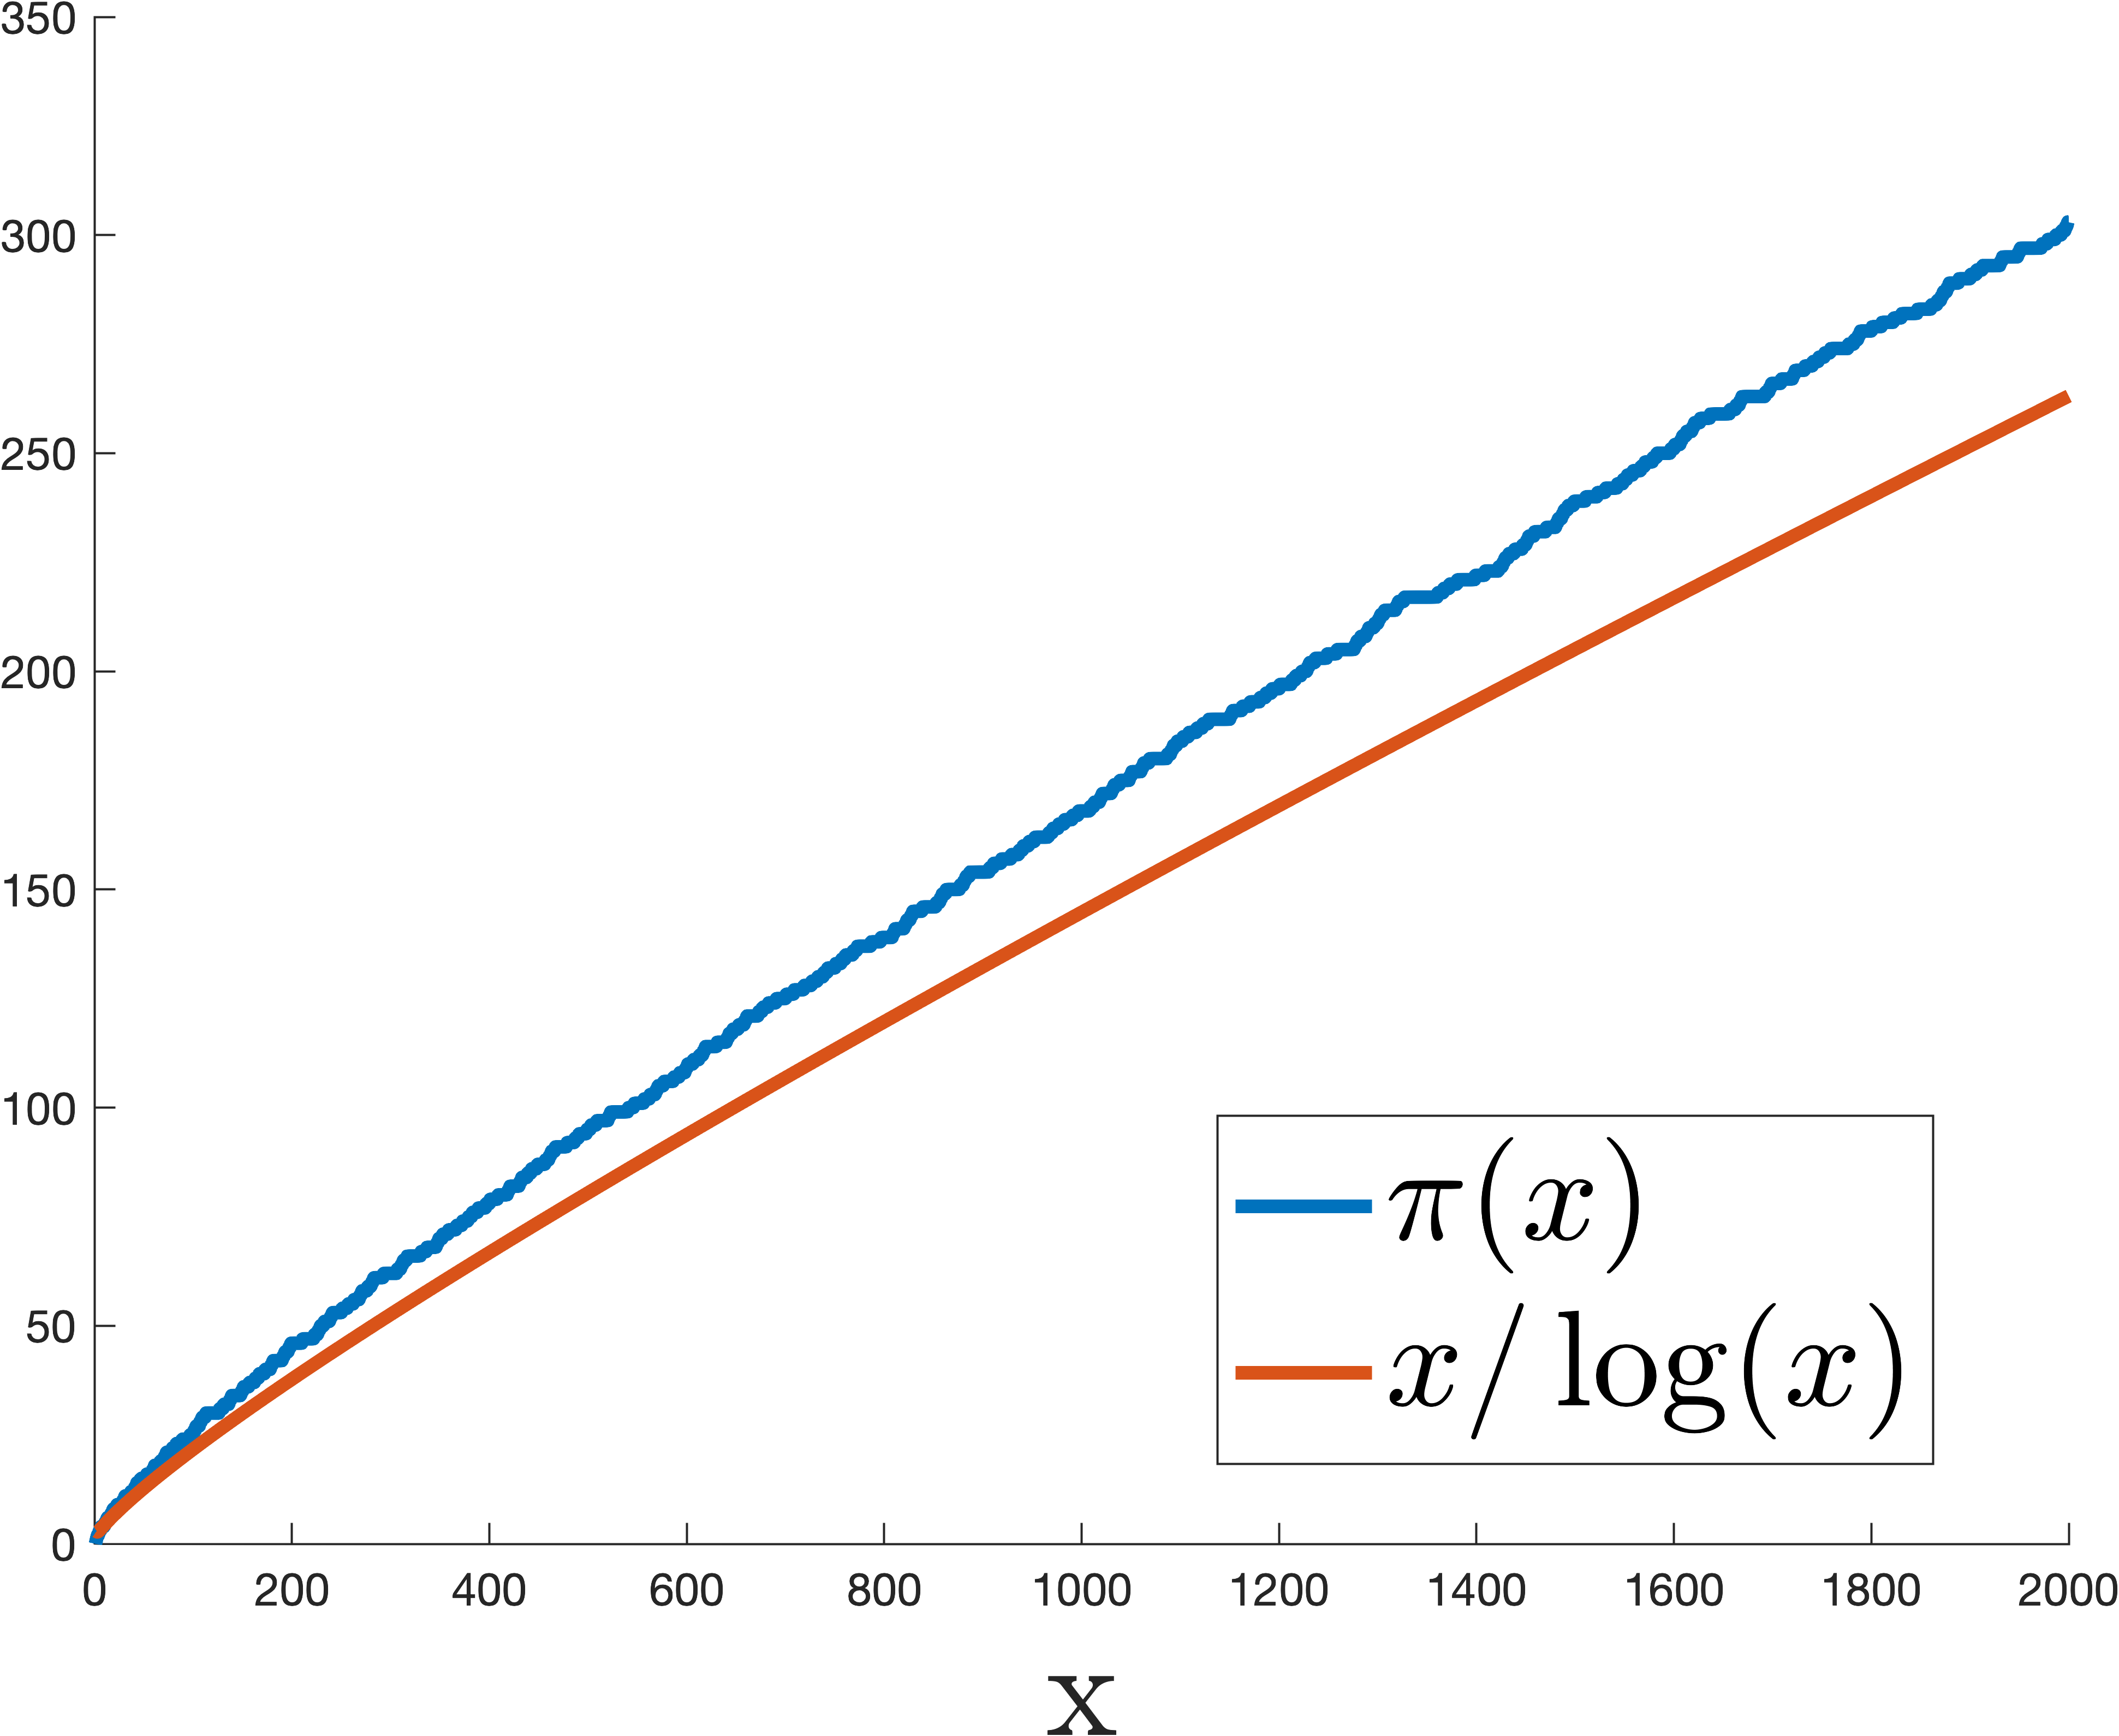
\includegraphics[width=.6\textwidth]{prime_number_theorem.png}
	\end{center}
\end{frame}

\begin{frame}
	\frametitle{prime number theorem}
	\textbf{Formally:}	For $x > 17$,
	\begin{align*}
		\frac{x}{\log(x)} \leq	\pi(x) \leq \frac{x}{\log(x) - 4}
	\end{align*}
	
	So if we select a random 128 bit number $p$, the chance that it is prime is great than:
	\begin{align*}
		\frac{1}{\log(2^{128})} \geq \frac{1}{90}
	\end{align*} 
	After a few hundred tries, we will almost definitely find a prime number. \textbf{In general, need $O(n)$ tries to find a prime with $n$ bits.}
\end{frame}

\begin{frame}
	\frametitle{prime numbers and hashing}
Finding large prime numbers is also a critical step in constructing efficiently computable universal hash. 

\textbf{Remainder of lecture:} Discuss a simple but really important application of prime numbers to hashing.
\end{frame}

\begin{frame}
	\frametitle{fingerprinting}
	\textbf{Goal:} Construct a compact ``fingerprint'' $h(f)$ for any given file $f$ with two properties:
	\begin{itemize}
		\item The fingerprints $h(f_1)$ and $h(f_2)$ should be different with high probability if the contents of $f_1$ and $f_2$ differ at all. 
		\item If the contents of $f_1$ and $f_2$ are identical, we should have $h(f_1) = h(f_2)$.
	\end{itemize}
	\begin{center}
		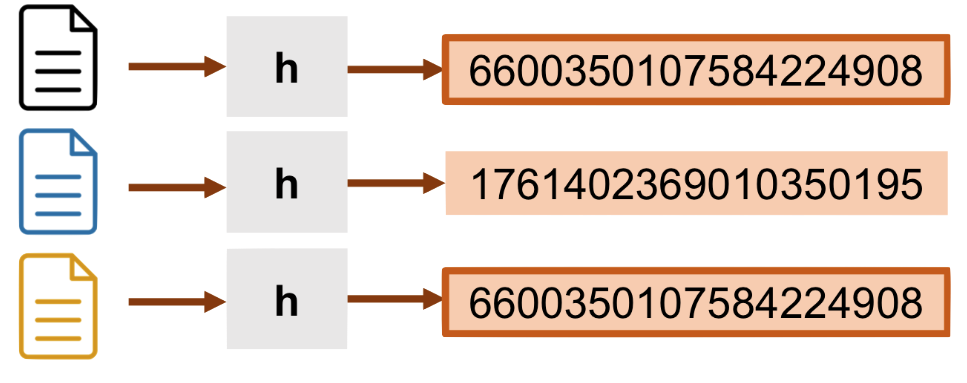
\includegraphics[width=.75\textwidth]{finger_print.png}
	\end{center}
\end{frame}

\begin{frame}[t]
	\frametitle{applications of finger printing}
	\begin{itemize} 
		\item Quickly check if two versions of the same file are identical (e.g. in version control systems like Git). Do not need to communicate the entire file between servers. Also used in webcaching and content delivery networks. 
		\item Check that a file pieced together from multiple parts is not missing anything. 
	\end{itemize}
	
\end{frame}

\begin{frame}[t]
	\frametitle{applications of finger printing}
	\begin{center}
		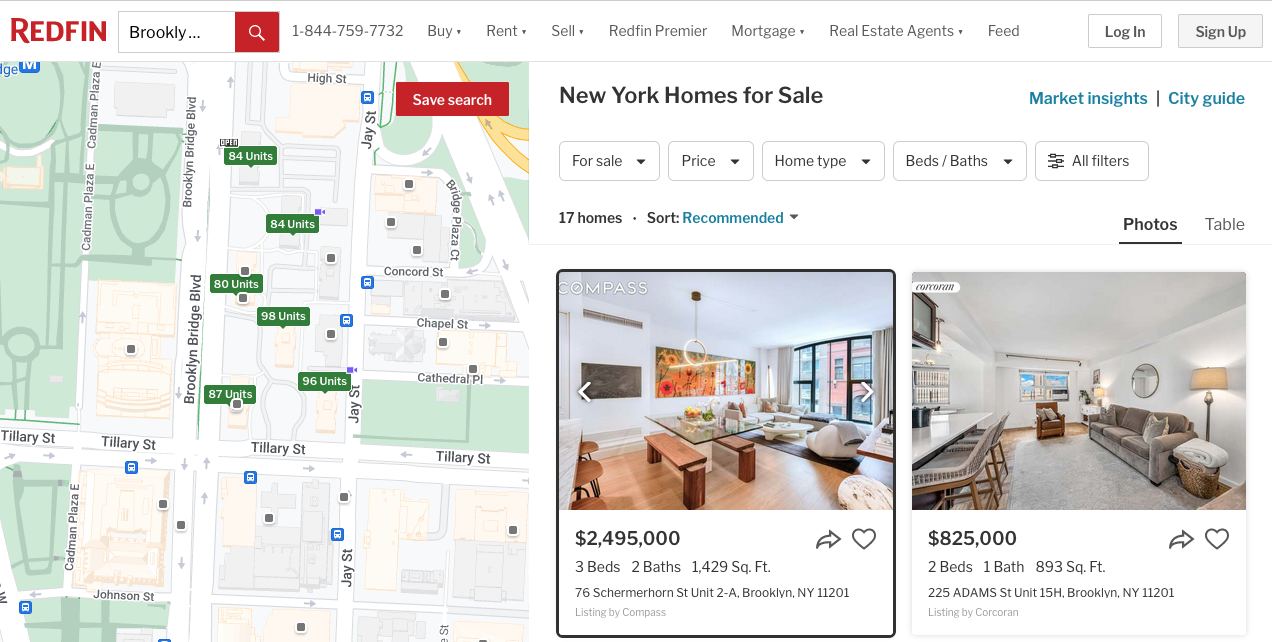
\includegraphics[width=\textwidth]{redfin_1.png}
	\end{center}
\end{frame}

\begin{frame}[t]
	\frametitle{applications of finger printing}
	\begin{center}
		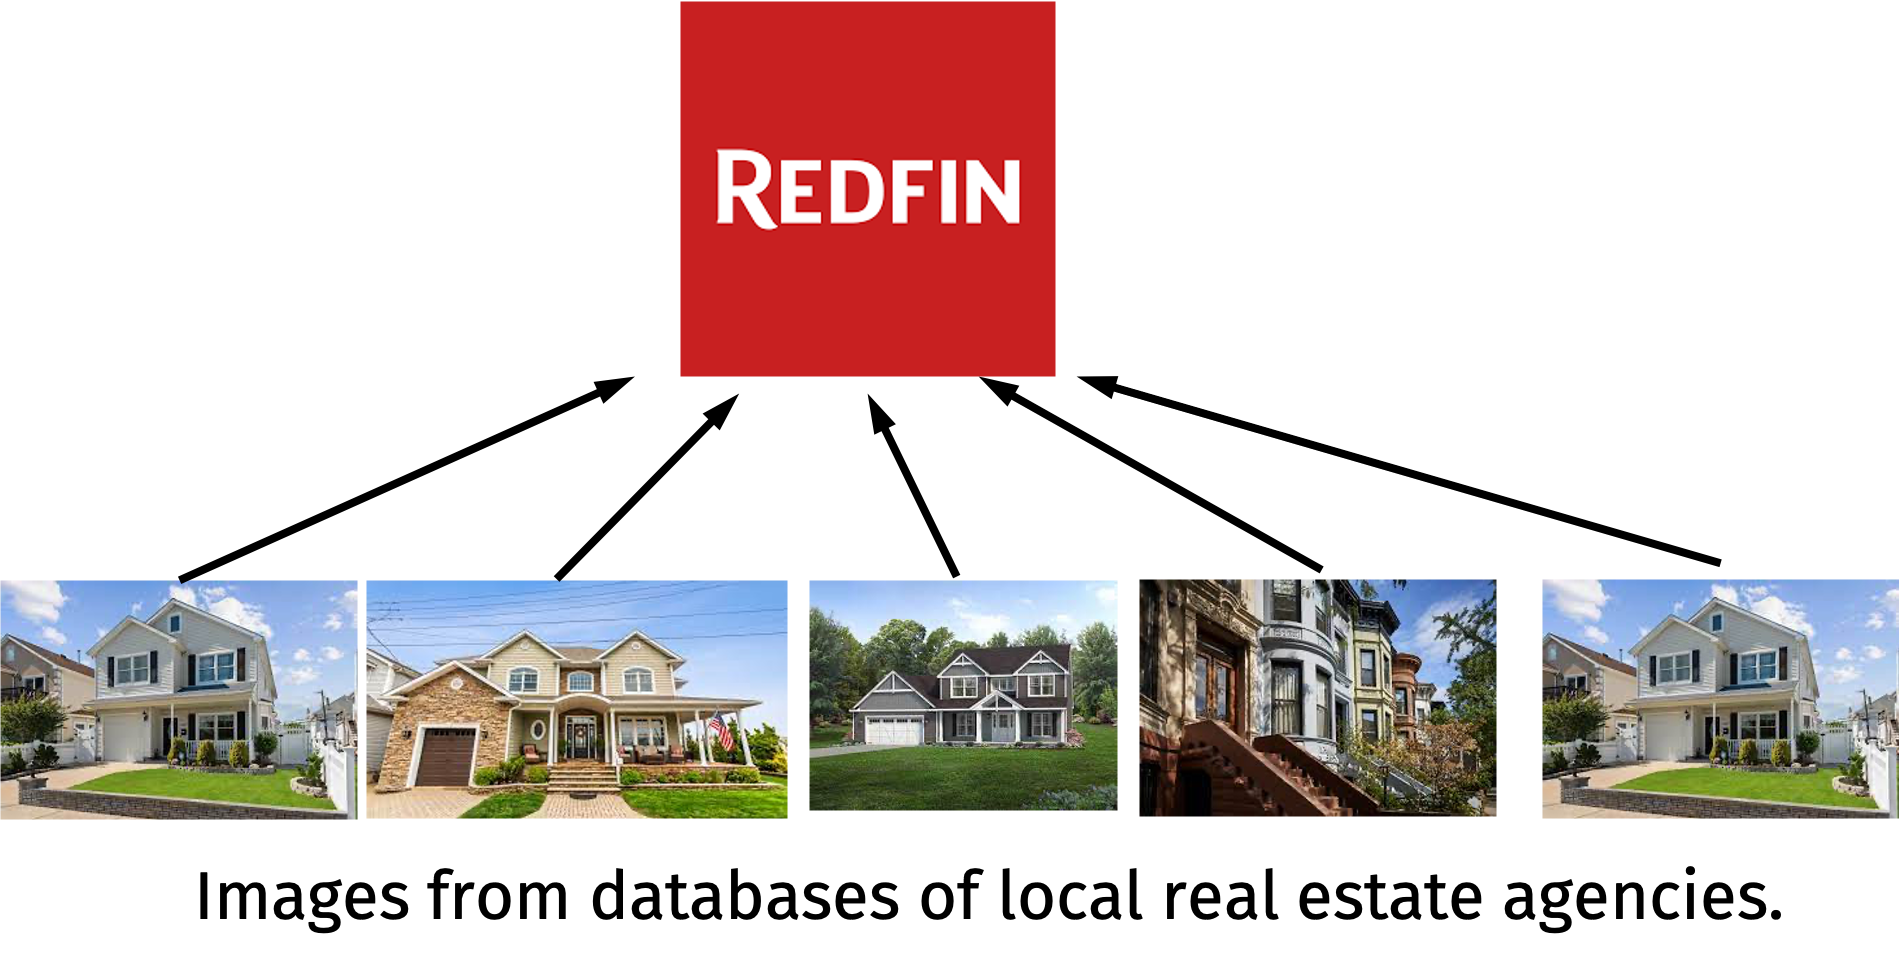
\includegraphics[width=\textwidth]{redfin_2.png}
	\end{center}
	
	Fingerprints used as file names for the images to make sure we did not reupload new images that we already had, and to detect duplicate images and listings.
\end{frame}

\begin{frame}
	\frametitle{fingerprinting}
	\textbf{Goal:} Construct a compact ``fingerprint'' function $h(f)$ such that:
	\begin{itemize}
		\item $h(f_1) \neq h(f_2)$ if $f_1 \neq f_2$ with high probability.
	\end{itemize}
\vspace{1em}
	Ideally, length of $h(f_1)$ (i.e. the size of the integers hashed to) is much less than the file size. 
\end{frame}

\begin{frame}
	\frametitle{random fingerprinting}
	\textbf{Rabin Fingerprint (1981)}: Let file $f = 010\ldots1101$ of length $n$ be interpreted as an $n$ bit integer. So something between $0$ and $2^n$. 
	
	\textbf{Construct $h$ randomly:} Choose random prime number $p$  between $2$ and $tn\log(tn)$ for a constant $t$.
	\begin{align*}
		h(f) = f \pmod{p}.
	\end{align*} 
	
	\begin{center}
		How many bits does $h(f)$ take to store?
	\end{center}
	
\end{frame}

\begin{frame}[t]
	\frametitle{random fingerprinting}
	\begin{align*}
		h(f) = f \pmod{p} \text{\hspace{1em} for prime } p\in \{2, \ldots, tn\log(tn)\}
	\end{align*} 
	\textbf{Claim:} If $f_1\neq f_2$ then $h(f_1) = h(f_2)$ with probability  $\leq \frac{2}{t}$.
	\vspace{3em}
	
	Since our fingerprint only takes $O(\log n + \log t))$ space,   we can  set $t$ to be \emph{super large}, so effectively the probability of $h(f_1)$ and $h(f_2)$ colliding is negligible for all real-world applications.
	
	E.g. set fingerprint length to $\log n + 28$ bits and you are more likely to win the Powerball.
\end{frame}


\begin{frame}[t]
	\frametitle{random fingerprinting}
	\begin{align*}
		h(f) = f \pmod{p} \text{\hspace{1em} for prime } p\in \{2, \ldots, tn\log(tn)\}
	\end{align*} 
	\textbf{Claim:} If $f_1\neq f_2$ then $h(f_1) = h(f_2)$ with probability just $\frac{2}{t}$.
	\vspace{3em}
	
	\textbf{First observation:} If $h(f_1) = h(f_2)$, then:
	\begin{align*}
		(f_1 - f_2) \pmod{p} = 0. 
	\end{align*}
	In other words, we only fail if \emph{the $f_1 - f_2$ is divisible by $p$}.
	
	
\end{frame}

\begin{frame}[t]
	\frametitle{random fingerprinting}
	\textbf{Question:} What is the chance that $f_1 - f_2$, which is an integer less than $2^n$, is divisible by a random prime $p\in \{2, \ldots, tn\log(tn)\}$?
	
\end{frame}

\begin{frame}[t]
	\frametitle{random fingerprinting}
	\textbf{Number of distinct prime factors of $f_1 - f_2$}: At most $n$.
	\vspace{1em}
	
	\textbf{Number of primes between $\{2, \ldots, tn\log(tn)\}$}: At least $\frac{tn\log(tn)}{\log(tn\log(tn))}$ via prime number theorem.
	
	\vspace{-1em}
	\begin{center}
		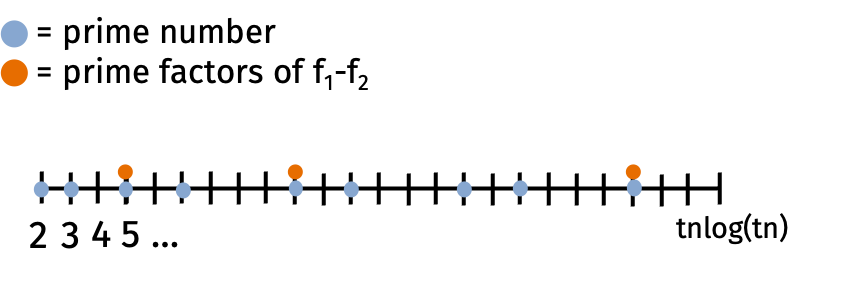
\includegraphics[width=\textwidth]{number_line.png}
	\end{center}
	\vspace{-1em}
Chance we pick a prime factor of $f_1 - f_2$ is less than:
	\begin{align*}
		\frac{n}{\frac{tn\log(tn)}{\log(tn\log(tn))}} =  \frac{\log(tn\log(tn))}{t\log(tn)} \leq \frac{2\log(tn)}{t\log(tn)}
	\end{align*}	
	
\end{frame}


\begin{frame}[t]
	\frametitle{random fingerprinting}
	\textbf{Conclusion:} The chance that a \emph{random} prime $p\in \{2, \ldots, tn\log(tn)\}$ is a factor of $f_1 - f_2$ is $\leq \frac{2}{t}$.
	
	So, for two files $f_1 \neq f_2$, the chance that $h(f_1) = h(f_2) \leq \frac{2}{t}$.
	\vspace{2em}
	
	Set $t = 10^{18}$ (the chance you win the Powerball twice in a row).
	
	\textbf{Fingerprint size:} At most $2\log_2(nt) = 2\log(n) + 2\log_2(10^{18})$ bits. 
	
	Suppose we are fingerprinting $1$mb image files. $n \approx 8\cdot 10^6$, so our fingerprint has size:
	\begin{align*}
		\alert{\mathbf{166}}\text{ \textbf{\alert{bits}}}
	\end{align*}
	
	This amounts to a \emph{50,000x reduction} over sending and comparing the original files.
\end{frame}

\end{document} 




